\documentclass[tikz,border=2mm]{standalone}

\begin{document}

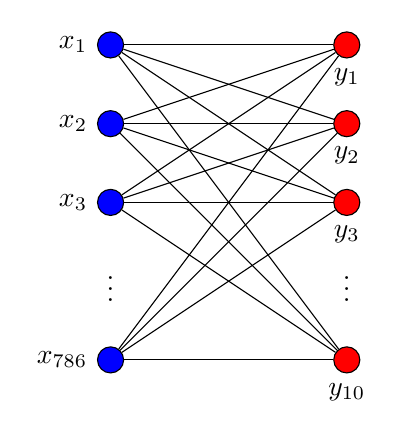
\begin{tikzpicture}
[   cnode/.style={draw=black,fill=#1,minimum width=3mm,circle},
]
    
    \node at (0,-4) {$\vdots$};
    \node at (3,-4) {$\vdots$};
    \foreach \x in {1,...,4}
    {   \pgfmathparse{\x<4 ? \x : "786"} 
        \node[cnode=blue,label=180:$x_{\pgfmathresult}$] (x-\x) at (0,{-\x-div(\x,4)}) {};        
        \pgfmathparse{\x<4 ? \x : "10"}
        \node[cnode=red,label=-90:$y_{\pgfmathresult}$] (p-\x) at (3,{-\x-div(\x,4)}) {};
        
    }
    \foreach \x in {1,...,4}
    {   \foreach \y in {1,...,4}
        {   \draw (x-\x) -- (p-\y);
        }
    }
\end{tikzpicture}

\end{document}